\section{Summary of Idea Forest}

The resulting forest was composed of 3007 instances, 1213 ideas, 335 category trees, and 129 non-singleton category trees. These metrics are decomposed by number condition is given in table TAB. A bird's eye view of the complete idea forest is in Figure FIG.

\begin{figure}[h!]
    \centering
    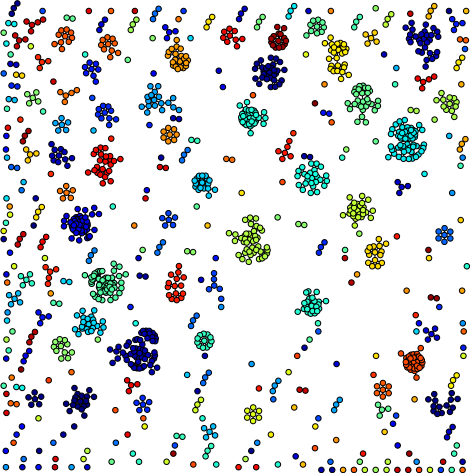
\includegraphics[width=0.9\columnwidth]{idea_forest}
    \caption{Idea Forest}
\end{figure}

\begin{table}
	\begin{tabular}[h!]{r | l l l l l l l}
	\textbf{number condition} & 5 & 10 & 20 & 50 & 75 & 100 & all \\ \hline \hline
	HITs & 57 & 47 & 23 & 10 & 10 & 10 & 146\\
	instances & 293 & 471 & 453 & 500 & 634 & 855 & 3007\\
	ideas & 171 & 249 & 278 & 341 & 443 & 177 &1212\\
	category trees & 72 & 79 & 93 & 114 & 172 & 177 &321\\
	non-singleton trees & 28 & 34 & 40 & 48 & 49 & 61 &92\\
	\end{tabular}
\end{table}

The height of category trees follows a roughly Poisson distribution, with the maximum tree height observed at 5. Summary statistics across condition are in table TAB. The third quartile drops as the number condition increases. While the upper conditions still discover categories trees with heights as great as 5, they generate many more "short" trees. This suggests that the ideas generated in the upper conditions are less common.

\begin{table}
	\begin{tabular}[h!]{r | l l l l l l l}
	\textbf{number condition} & 5 & 10 & 20 & 50 & 75 & 100 & all \\ \hline \hline
	median & 2 & 2 & 2 & 2 & 2 & 2 & 2\\
	first quartile & 2 & 2  & 1 & 1 & 1 & 1 & 1\\
	third quartile & 3 & 3 &3 &3 &2 &2 & 2\\
	\end{tabular}
	\caption{Category tree height}
\end{table}

The number of nodes and number of instances are also roughly Poisson distributed (Table TAB). In keeping with the findings for height, trees found in the upper number conditions are smaller than trees found in the lower conditions. The precipitous drop in median tree size suggests that in the largest condition, participants are finding rare ideas with only a few variants and less than 14 instances.

\begin{table}
\begin{tabular}[h!]{r | l l l l l l l}
	\textbf{number condition} & 5 & 10 & 20 & 50 & 75 & 100 & all \\ \hline \hline
	number of nodes& \\ \hline
    median &5&5&4&3&2&2&2 \\
	first quartile &2&2&1&1&1&1&1 \\
	third quartile &17&17&14&10&5&5&5 \\
	number of instances& \\ \hline
	median &14&14&12&10&4&4&4 \\
    first quartile &4&4&4&2&1&1&1 \\
	third quartile &47&45&30&23&13&13&13 \\
	\end{tabular}
	\caption{Number of ideas and instances in trees}
\end{table}

To better understand what this distribution of tree sizes means...
